% !TEX root = ../thesis-example.tex
%
\chapter{Related work}
\label{chapter2}

\section{State of the Art}

As for mobile systems, there are only two main platforms: Android and iOS. On the Android side, because of it being an open source project, a vast number of smartphone manufacturing companies provide this base operating system and some have even implemented their own wrapper around Android. As a result, the device suite for Android has surpassed 7000+ devices [4]. On the other hand, the iOS platform is much more restrictive and only Apple is allowed to manufacture devices with iOS, which results in the testing advantage of having a smaller device suite [3]. However, due to the secrecy and restrictions of the iOS system (as opposed to Android), there are fewer tools available that may perform automated tests, making test automation fairly more uncommon on this platform. Consequently, test assessment might be performed through manual testing instead of automated even if automating is the right approach.

There are currently a few tools that allow the development of automated user interface tests for iOS. The feasibility of developing tests through one or the other varies depending on the compatibility of the tool with the characteristics of the project. This refers to features such as: the programming language with which the team to perform the automation is familiar with, which testing framework are you capable of using, if the application is developed hybrid or native, the testing load and speed requirements, among many others.

The two types of tools used to create automated tests are: Automation APIs/frameworks and record and replay tools [9]. It is also worth noting that there are several test support tools like: bug and error reporting/monitoring tools, device streaming tools and automated test input generation tools. For the purpose of this project, a focus on both types of test automation tools will be made: APIs/frameworks and record and replay.

First, it is important to provide an overview on how these two tool types work and how they are used to create automated tests. Under the hood, they work in a very similar manner and even, in some cases, test automation systems provide both tools. In order to create automated tests for mobile applications there is a crucial feature the tool must provide. The tool needs to be capable of interacting with the smartphones GUI elements as a real user would in order to replicate testing scenarios. This includes GUI interactions such as: swiping, typing, pinch and zoom, tapping among others and even combinations of these like swipe and hold or double tap. Even though both tool types must provide this interaction with the GUI, the way the actual automated tests are created is where they differ. Automation APIs/frameworks require a test script which contains all of the user interactions that should be performed when the test is to be executed. On the other hand, record and replay tools only require for the test to be manually executed and the tool itself will record all the interactions that where performed generating a test script.


\section{Test Automation Tools}

Regarding the available tools, there are several different tools that can be used to develop your automated tests, ranging from paid license all-in-one tools like Ranorex [7] to open source client server tools like Appium [8], which acts as a library that you can adapt to your test automation framework. 

Getting to know all of the available tools, how they work and how they are used can become a very time-consuming task. Besides, while doing research about test automation tools for iOS, you might end up with a small list of the available tools and a brief understanding of them. The actual documentation you can find on automation tools for iOS is very limited and as a result you can easily have a hard time trying to choose the appropriate tool for your project. For this reason, this project pursues to reduce the conceptual gap present when trying to learn about the available user interface test automation tools for iOS.

Here, a list and a brief description for most of the currently available tools that may perform test automation of UI over the iOS platform is shown. This will provide a high level view of what is available and may help you discard some options right away.

\subsection {XCTest UI}
Xcode comes with the testing framework XCTest. This testing framework will not only allow you to code your unit tests, but you may also record and write UI tests. This testing tool has seen a mayor upgrades since it was released a few years ago and has now become a really solid option.

\subsection {Appium}
Appium has now become one of the most popular mobile test automation tools out there. This open source project is characterized by its client server architecture which supports a wide range of programming languages and testing frameworks to work on.

\subsection {Calabash}
Although Xamarin (Microsoft) discontinued their development for this test automation framework up until iOS 11 and Android 8, it has still been maintained by its community. It works with Cucumber in order to follow the BDD practices plus it is a free and open source project. This means it can become fairly simple to write automated tests without much coding experience.

\subsection {Earl Grey (2.0)}
This open source project by Google provides a testing framework over the existing XCUITest in order to provide certain advantages such as synchronization and white box testing.
	
\subsection {Ranorex}
This paid “all in one” solution seems to be one of the most popular of its kind. It allows the recording and writing of automated tests for many platforms and it is simple to use, for which its users do not need to be skilled with programming to use it.

\subsection {KIF}
KIF, standing for “Keep It Functional” is a test automation framework that works at the XCTest level and runs with your unit tests. Tests are written in Objective-C and it is characterized for being simple and easy to use.

\subsection {Detox}
Detox is a grey-box end to end testing framework for mobile devices (iOS and Android) which provides fast tests with improved reliability regarding flakiness. It is designed to support both React Native and pure native ones and it may perform testing over a real device or a simulator.

\subsection {Frank}
This BDD automated acceptance testing framework works with cucumber and provides features such as recording your tests and running on both simulator and real devices.

\subsection {TestComplete}
This paid all in one solution provides everything you may need in order to build and run your tests ranging from the testing framework to the physical/virtual devices. You can either write your own tests on any of the 7 available languages or use the built-in record and replay tool.

\subsection {MonkeyTalk}
MonkeyTalk is a record and replay open source mobile app automation tool. It is very simple to setup and use, plus it supports both android and iOS.

\subsection {Quantum}
The Quantum framework allows you to build BDD automated tests using cucumber. It supports both iOS and Android. Tests are written in Java.

\section{Comparison Table}
In the following table you will be able to visualize a comparison between the main characteristics of the previously mentioned tools. Further on, the study case will provide even more specific information about a few of these tools.

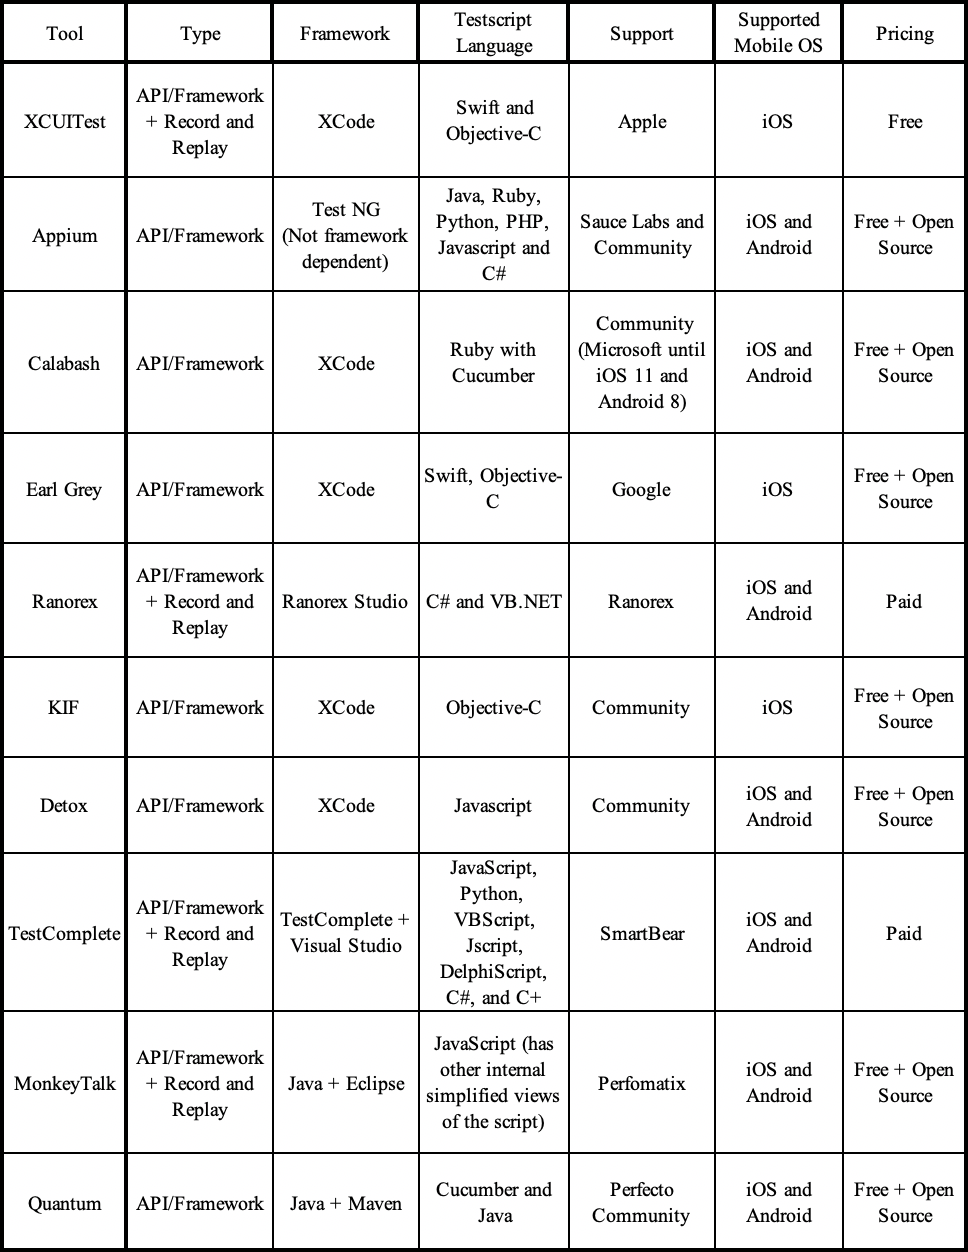
\includegraphics[width=12cm]{img/table1.png} \\[2mm]

\section{Categories}
In order to compare test automation tools, it is important to understand the different elements, interactions and functionality an iOS mobile app utilizes. These will be broken down in three categories: GUI components, Gestures and Testing Capabilities. The first makes reference to the all the elements that make up the graphical user interface, these are also divided into three categories: Bars, Views and Controls. Gestures are the way users interact with the touchscreen, this is the main way users provide input to their mobile devices. Finally, testing capabilities make reference to the various APIs the test automation tool could provide in order to manipulate the application OS and hardware configurations.

The following is a list of GUI components and gestures Apple has publicly defined [To-Link], as well as some of the testing capabilities that one may need while automating tests. 

\subsection {GUI Components}
	
	Bars
	\begin{itemize}
  		\vspace{-0.4cm}\item Navigation Bar
  		\vspace{-0.4cm}\item Search Bars
		\vspace{-0.4cm}\item Status Bars
		\vspace{-0.4cm}\item Tab Bars
		\vspace{-0.4cm}\item Toolbars
	\end{itemize}

	Views
	\begin{itemize}
  		\vspace{-0.4cm}\item Action Sheets
		\vspace{-0.4cm}\item Activity Views
		\vspace{-0.4cm}\item Alerts
		\vspace{-0.4cm}\item Collections
		\vspace{-0.4cm}\item Image Views
		\vspace{-0.4cm}\item Pages
		\vspace{-0.4cm}\item Popovers
		\vspace{-0.4cm}\item Scroll Views
		\vspace{-0.4cm}\item Split Views
		\vspace{-0.4cm}\item Tables
		\vspace{-0.4cm}\item Text Views
		\vspace{-0.4cm}\item Web Views
	\end{itemize}
	
	Controls
	\begin{itemize}
  		\vspace{-0.4cm}\item Buttons
		\vspace{-0.4cm}\item Context Menus
		\vspace{-0.4cm}\item Edit Menus
		\vspace{-0.4cm}\item Labels
		\vspace{-0.4cm}\item Page Controls
		\vspace{-0.4cm}\item Pickers
		\vspace{-0.4cm}\item Progress Indicators
		\vspace{-0.4cm}\item Refresh Content Controls
		\vspace{-0.4cm}\item Segmented Controls
		\vspace{-0.4cm}\item Sliders
		\vspace{-0.4cm}\item Steppers
		\vspace{-0.4cm}\item Switches
		\vspace{-0.4cm}\item Text Fields
	\end{itemize}

\subsection {Gestures}

	\begin{itemize}
  		\vspace{-0.4cm}\item 3D Touch
		\vspace{-0.4cm}\item Tap
		\vspace{-0.4cm}\item Drag
		\vspace{-0.4cm}\item Flick
		\vspace{-0.4cm}\item Swipe
		\vspace{-0.4cm}\item Double tap
		\vspace{-0.4cm}\item Pinch
		\vspace{-0.4cm}\item Touch and Hold
		\vspace{-0.4cm}\item Shake
		\vspace{-0.4cm}\item Rotate
	\end{itemize}

\subsection {Framework Testing Capabilities}
	\begin{itemize}
  		\vspace{-0.4cm}\item Element handling: Element searching and Element attributes
		\vspace{-0.4cm}\item Authentication: Touch ID and Face ID
		\vspace{-0.4cm}\item Toggle hardware configurations: Wi-Fi, Data, Bluetooth, …
		\vspace{-0.4cm}\item Access system configurations: Language, Region, Time, Text Size, …
		\vspace{-0.4cm}\item Change device orientation
		\vspace{-0.4cm}\item GPS mocking
		\vspace{-0.4cm}\item Camera mocking
		\vspace{-0.4cm}\item Application state (set app to background, reopen app)
		\vspace{-0.4cm}\item Multitasking
		\vspace{-0.4cm}\item Notification handling
		\vspace{-0.4cm}\item Access app cache  data
		\vspace{-0.4cm}\item File handling
	\end{itemize}
	
\subsection {Automation Tool Characteristics and Features}

Another important aspect to take into account when evaluating the suitability of a framework for a project is the characteristics and features the tool provides. There are certain characteristics or features besides the automated testing itself that may become invaluable. 

Examples for such are: 
	\begin{itemize}
  		\vspace{-0.4cm}\item Performance: Test execution time, memory use, …
		\vspace{-0.4cm}\item Maintainability
		\vspace{-0.4cm}\item Test parallelization
		\vspace{-0.4cm}\item Emulated and Real Device compatibility
		\vspace{-0.4cm}\item Ease of development (skill required)
		\vspace{-0.4cm}\item Android (hybrid) project compatibility
		\vspace{-0.4cm}\item Programming Languages Supported
		\vspace{-0.4cm}\item Developer Support
		\vspace{-0.4cm}\item Price
	\end{itemize}

